\chapter{Introduction}

\section{Non Linearity}
Per estendere i modelli lineari a funzioni non lineari possiamo applicare una trasformazione non lineare $\phi(x)$ all'input.

La funzione $\phi(x)$ definisce una nuova rappresentazione di $x$.

La funzione $\phi(x)$ può essere generica come nelle \textit{kernel machines} oppure può essere imparata aggiornando i parametri $\theta$.
\begin{flalign*}
  &\quad f(x; \theta; \omega) = \phi(x; \theta)^T\omega \: \text{,}&
\end{flalign*}
dove $\theta$ sono i parametri e $\omega$ i pesi del modello.

Una rete con 1 hidden layer può imparare una qualsiasi funzione $f(x)$ non lineare.
La difficoltà consiste nel trovare i pesi per determinare $f(x)$.

\pagebreak

\subsubsection*{XOR Example}
XOR function: $y = f^*(x)$

$X = \{[0, 0]^T, [0, 1]^T, [1, 0]^T, [1, 1]^T\}$

$y = f(x; \theta) \Rightarrow f^*(x)$

Supponiamo di scegliere un mapping lineare $f(x; \theta)= f(x; \omega, b) = x^T\omega +b$

\begin{minipage}[c]{0.4\textwidth}
  \newcommand{\x}[2]{$x_#2$}
  \newcommand{\h}[2]{$h_#2$}
  \newcommand{\y}[2]{y}
  \newcommand{\Input}[2]{x}
  \newcommand{\Hidden}[2]{h}
  \newcommand{\w}[4]{w}
  \newcommand{\W}[4]{$\omega$}

  \vspace{0pt}\
  \begin{neuralnetwork}[layerspacing=18mm]
    \inputlayer[count=2, bias=false, text=\x]{}
    \hiddenlayer[count=2, bias=false, text=\h]{} \linklayers
    \outputlayer[count=1, text=\y]{} \linklayers
  \end{neuralnetwork}

  \bigskip

  \vspace{0pt}\
  \begin{neuralnetwork}[layerspacing=18mm]
    \inputlayer[count=1, bias=false, text=\Input]{}
    \hiddenlayer[count=1, bias=false, text=\Hidden]{} \linklayers[labels=\w]
    \outputlayer[count=1, text=\y]{} \linklayers[labels=\W]
  \end{neuralnetwork}
\end{minipage}
\hfill
\begin{minipage}[s]{0.55\linewidth}
  \noindent
  \begin{flalign*}
    &h = f^{(1)}(x; w, c)&\\
    &y = f^{(2)}(h; \omega, c)&\\
    &f(x; w, c, \omega, b) = f^{(2)}(f^{(1)}(x))&\\
    &f(x; w, c, \omega, b) = max\{0, xw + c \} \; \omega + b&
  \end{flalign*}
\end{minipage}

%
Supponiamo di inizializzare i parametri nel seguente modo:
\begin{flalign*}
  &w =
  \begin{bmatrix}
    1 & 1 \\
    1 & 1 \\
  \end{bmatrix}
  \;
  c =
  \begin{bmatrix}
    0  \\
    -1 \\
  \end{bmatrix}
  \;
  \omega =
  \begin{bmatrix}
    1  \\
    -2 \\
  \end{bmatrix}
  \;
  b =
  \begin{bmatrix}
    0 \\
    0 \\
  \end{bmatrix}&
\end{flalign*}

\begin{flalign*}
  &max(0, xw + c)\; \omega = [0, 1, 1, 0]^T&
\end{flalign*}

Multi-Layer Neural Networks:
\begin{itemize}
  \item Feed Forward Neural Network (FFNN)\\
        non hanno connessioni che formano loop
  \item Recurrent Neural Network (RNN)\\
        hanno loop, utili per informazioni sequenziali
  \item Convolutional Neural Network (CNN)\\
        catturano informazioni spaziali attraversi molteplici filtri
\end{itemize}


\begin{figure}[ht]
  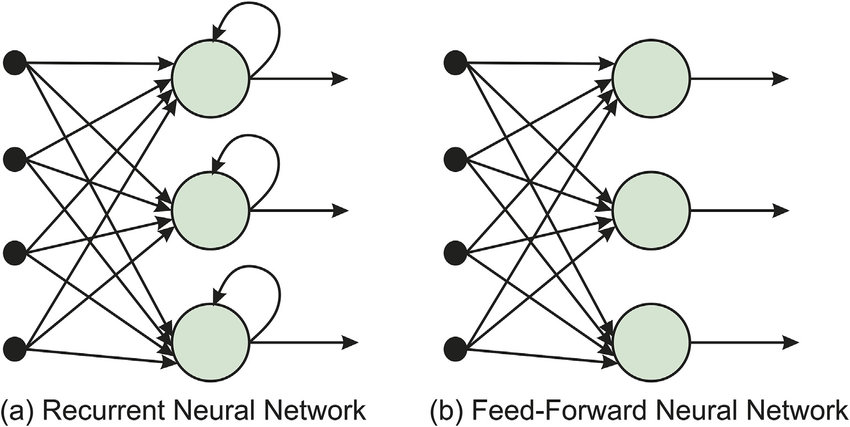
\includegraphics[width=.475\textwidth]{images/The-comparison-between-Recurrent-Neural-Network-RNN-and-Feed-Forward-Neural-Network.jpg}
  \hfill
  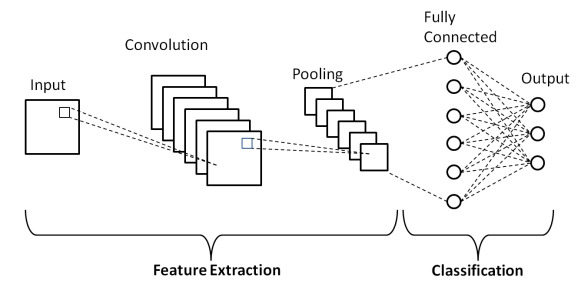
\includegraphics[width=.475\textwidth]{images/Schematic-diagram-of-a-basic-convolutional-neural-network-CNN-architecture-26.jpeg}
  \caption{Differenza tra RNN, FFNN \cite{img:rnn-ffnn} e CNN \cite{img:cnn-architecture}}
\end{figure}

\section{Feed Forward Neural Network}
Una FFNN è una rete fully connected, ovvero che ogni neurone in un layer e collegato a tutti gli altri del layer successivo.
Una FFNN può essere pensata come una concatenazione di funzioni applicate all'input $x$, $f(x) = f^{(3)}(f^{(2)}(f^{(1)}(x)))$.

La lunghezza della catena corrisponde alla \textbf{depth} del modello. La dimensionalità degli hidden layer determina la \textbf{width} del modello.

Il training del modello consiste nel trovare una funzione $f(x)$ che si avvicini il più possibile a una funzione target $f^*(x)$. $f(x) \rightarrow f^*(x)$.
